\documentclass[11pt]{article}
\usepackage[margin=0.8in]{geometry}
\usepackage{amsmath,amssymb,graphicx,hyperref}
\setlength{\parindent}{0pt}\setlength{\parskip}{6pt}
\setlength{\emergencystretch}{3em}
\begin{document}
{\Large Public branch coordinates and derived cofactor guards}\par
2026-11-13. Unsigned producer evidence [pcc:unverified].

The actual polynomial branch now has explicit public coordinates. Restricting
the actual quotient-moment matrix through them yields numerical corank one
and a nonzero diagonal adjugate entry under the exact prior chart hypotheses.
Those conditions are derived, rather than supplied as numerical rank guards.
Frozen source \path{01e312a94d}; module \path{NormBranchCoordinates}.

\textbf{Public map.} Put $a=\deg F$, $b=\deg H$, $N=(a+1)+(b+1)$,
$n=N-1$. The actual product monomial families give
$\ell_i=A_i(q)-yB_i(q)$ and $\ell_0=1$, since the first pair is $(1,0)$.
Define
\[
 Tz=\left(-\sum_{j=0}^{n-1}\ell_{j+1}z_j,\ z_0,\ldots,z_{n-1}\right),
 \qquad Lw=(w_1,\ldots,w_n).
\]
Then $LT=I$, $TLw=w$ on $\ker\ell$, and $\ell(Tz)=0$. The columns of $T$
are public; no witness or basis-selection oracle is used. Define the actual
reduction $S_{\rm red}=T^{\mathsf T}ST$. Its entry formula is
\[
 (S_{\rm red})_{ij}=S_{i+1,j+1}-\ell_{i+1}S_{0,j+1}
 -\ell_{j+1}S_{i+1,0}+\ell_{i+1}\ell_{j+1}S_{00}.
\]
The arbitrary-pair identity is proved for this actual congruence [pcc:unverified].

\textbf{Exact hypotheses.} Over any field: $F,H$ monic, $\deg H>0$,
$\deg H+1<\deg F$, $UF+V(fH)=1$, $F(q)\ne0$, $\alpha\ne0$, and
$\alpha F(q)-y\beta H(q)=0$. These are the prior quotient-moment chart
assumptions, not a new class of prime-field curves.

\begin{center}
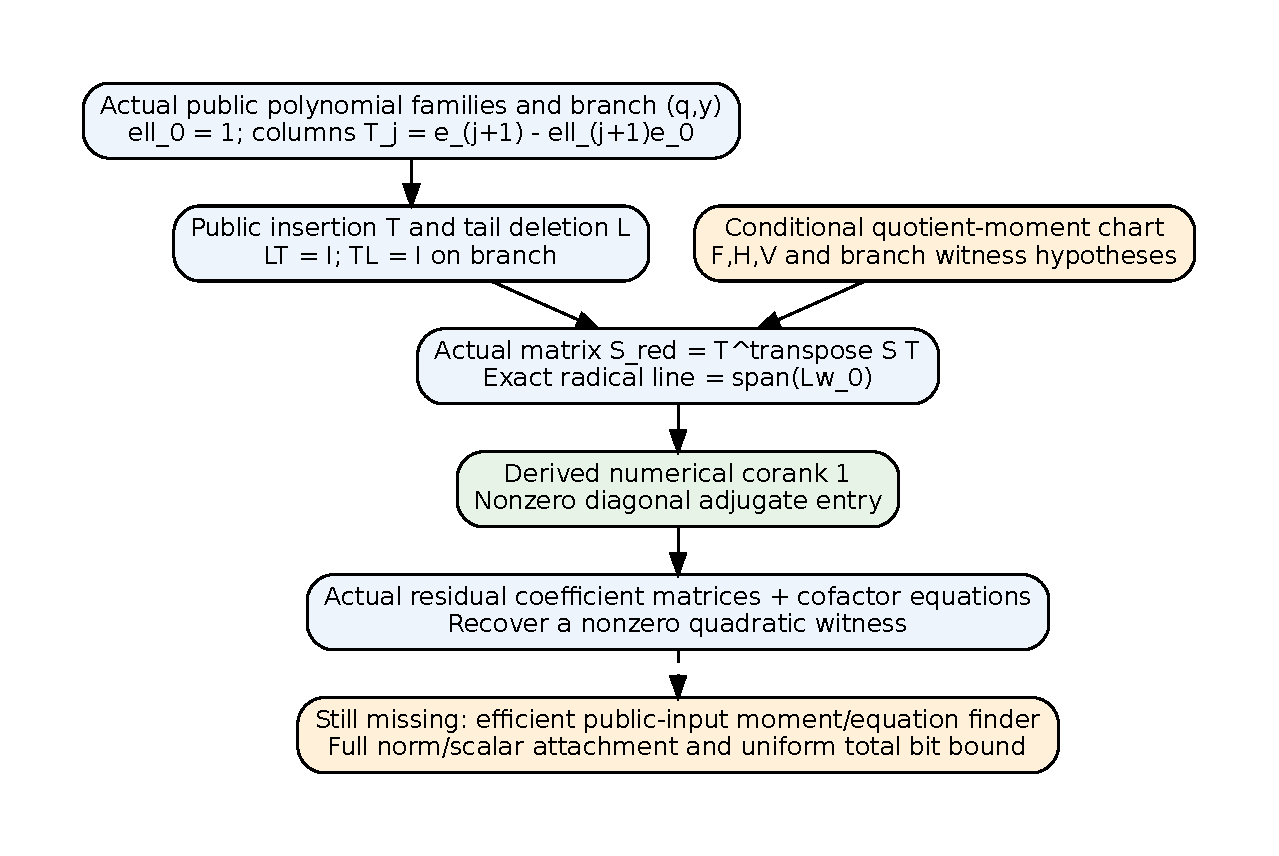
\includegraphics[width=\linewidth,height=0.33\textheight,keepaspectratio]{coordinates.pdf}
\end{center}

\textbf{Actual radical.} For $S$ from the actual functional
$\operatorname{moment}(F,V)$, its reduced left radical is exactly
$\operatorname{span}(Lw_0)$, where $w_0$ represents $(\alpha F,\beta H)$.
Completeness constructs these coordinates; the branch inverse proves
$Lw_0\ne0$. Rank-nullity gives $\operatorname{rank}S_{\rm red}+1=n$, hence
$\det S_{\rm red}=0$. No literal unrelated matrix is substituted [pcc:unverified].

\newpage
{\Large Nonzero cofactor, actual recovery and remaining search}\par

\textbf{Explicit cofactor.} In a symmetric matrix with the proved radical
line, choose $k$ at a nonzero radical coordinate. Replace row $k$ by $e_k$.
A vector in this updated kernel has coordinate $k$ zero and satisfies all
other original rows. Pairing with the radical forces the missing row too.
Symmetry places the vector in the radical line, so it must be zero. The
updated matrix is invertible; its determinant is exactly the diagonal
adjugate entry $(\operatorname{adj}S_{\rm red})_{kk}\ne0$. No nonzero-minor
oracle or division by 2 is assumed. This is standard linear algebra
[pcc:unverified].

\textbf{Actual coefficient recovery.} For $j<\deg G$, use
\[
 \mu_j(P)=P_j-P_{\deg G}G_j,\qquad
 Q_{{\rm red},j}=T^{\mathsf T}Q_jT.
\]
If every pairing $\langle Q_{{\rm red},j},\operatorname{adj}S_{\rm red}\rangle$
vanishes, the instantiated recovery theorem gives $x\ne0$ with
$x^{\mathsf T}Q_{{\rm red},j}x=0$ for all these actual coefficient matrices.
Its symmetry, determinant, corank and adjugate guards are derived. The
conclusion is quadratic conditions; a nonzero normalized norm scalar,
complete divisor/scalar recovery and their degree-chart attachment remain
further obligations.

\begin{center}\small
\begin{tabular}{ll}
Exact component & Declaration in \path{NormBranchCoordinates}\\\hline
First actual coefficient & \path{actualFirstCoefficient}\\
Public inverse maps & \path{deleteInsert}, \path{insertDelete}\\
Actual reduced radical & \path{actualReducedRadical}\\
Numerical corank/determinant & \path{actualReducedCorank}, \path{actualReducedSingular}\\
Nonzero actual cofactor & \path{actualReducedCofactor}\\
Actual coefficient recovery & \path{actualCoefficientRecovery}
\end{tabular}\end{center}

\textbf{Verification.} There are 25 new theorem statements. The whole-study
tracked-source gate audits 201 statements with 0 additional trusted axioms.
All 25 print only propext, Classical.choice and Quot.sound. Import-inclusive
fresh replay has its separate completion receipt. These are producer checks;
independent signed PCC standing is not asserted. Canonical source bindings,
all failed/successful logs and exact pins accompany this report.

\textbf{Failures retained.} Builds 001--009 fail on index annotations, partial
application, matrix constructor recognition, export opacity and quantified
index conversion. Build 010 first passes the actual radical; 011--014 add rank,
actual corank, cofactor pivot and actual cofactor. Build 015 passes the final
25 statements without a new-module warning. A failed stage printing sorryAx
is never counted as a proof. No solver, timing or paid run; no benchmark edit.

\textbf{Finder gap.} Suitable $F,H,V$/moments and the cofactor equations are
still supplied. Efficiently finding them from public ECDLP input, actual norm
recovery and uniform total bit cost remain open. Reachability through the
annotated $W_{\rm base}+C(T)H(T)$ jet corrections is separate; its $H$ is not
the norm polynomial by naming alone.

\textbf{Sources.} Prior actual family, moment and branch modules; explicit basis
plan; pinned Mathlib polynomial bases, finite tuples/sums, matrix products,
ranks, row updates, adjugates, invertibility and rank-nullity. Exact paths are
in the companion README. KB unavailable; no exhaustive review or novelty
claim. Live compute admission unobserved.
\end{document}
